% double-cone-sharp-nose.tex

\section{Hypersonic flow over a double-cone.}
\label{sec:double-cone-sharp-nose}
%
This is another of the hypersonic test flows provided by the Calspan-University of Buffalo Research Center (CUBRC)
as part of an experimental campaign\,\cite{holden_etal_2002a,holden_wadhams_2003a} in the LENS shock tunnel at CUBRC.
The experimental facility provides a Mach 12.49 flow of nitrogen along the cylinder with flare shown below 
in Figure\,\ref{fig:double-cone-sharp-nose-model}.
As for the hollow-cylinder with flare case in Section\,\ref{sec:cylinder-flare}, 
it is an example that retains a very simple geometric arrangement for the flow boundaries, however, 
the stronger shock interaction with the steeper cone surface produces a more complex flow.
Despite this complexity, the overall flow eventually settles to a steady state and 
we assume that the boundary layer remains laminar.

\begin{figure}[htbp]
 \centering
 \subfloat[Physical model.]{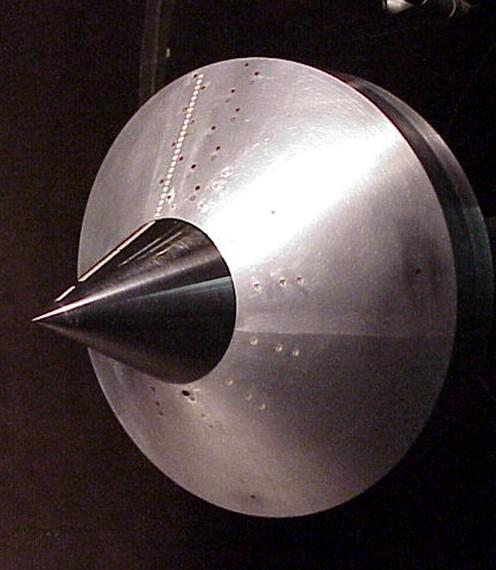
\includegraphics[width=0.40\textwidth]
  {../2D/double-cone-sharp-nose/notes/double-cone-sharp-nose-CUBRC-photo.jpeg}}
 \subfloat[Geometric definition from \cite{maclean_holden_2004a}.  Dimensions in inches and mm.]
  {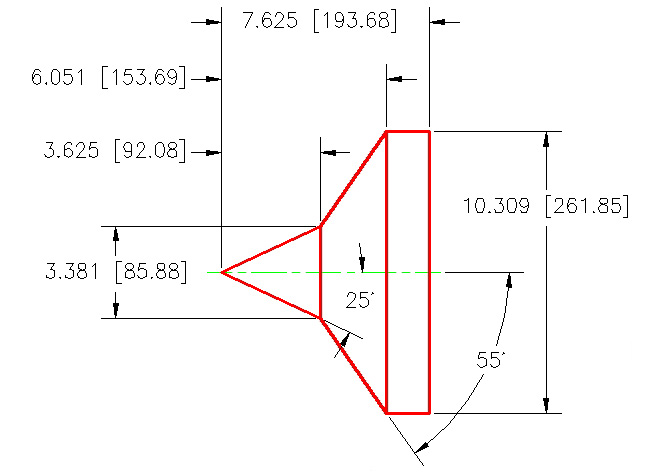
\includegraphics[width=0.60\textwidth]
   {../2D/double-cone-sharp-nose/notes/maclean-2004-0529-figure-2a.png}}
 \caption{Double-cone with sharp nose used in the CUBRC experiments.}
 \label{fig:double-cone-sharp-nose-model}
\end{figure}

\bigskip
\subsection{Input script (.py)}
%
In setting up this exercise, we follow the details provided by MacLean\,\cite{maclean_holden_2004a}
and concentrate on the CUBRC Run 35 experiment.
We assume an ideal nitrogen free stream, with conditions 
$p$ = 18.55\,Pa, $\rho$=0.6081\,g/m$^3$, $u$ = 2.576\,km/s and a static temperature $T$=102.2\,K.
The actual nitrogen flow in the shock tunnel nozzle was far from ideal and had an estimated
vibrational temperature of 2711\,K.
However, for the simulation reported here, this vibrational energy is assumed frozen and thus ignored.
The model surface temperature was a constant 295.8\,K.

\noindent
\topbar
\lstinputlisting[language={}]{../2D/double-cone-sharp-nose/dbl-cone.py}
\bottombar


\bigskip
\subsection{Running the simulation}
%
Figure\,\ref{fig:double-cone-sharp-nose-geometry} shows the flow region, as modelled for simulation.
The region is very simple but we have divided it into 28 blocks so that the computational load 
can be shared across a number of CPU cores.

\begin{figure}[htbp]
 \centering
 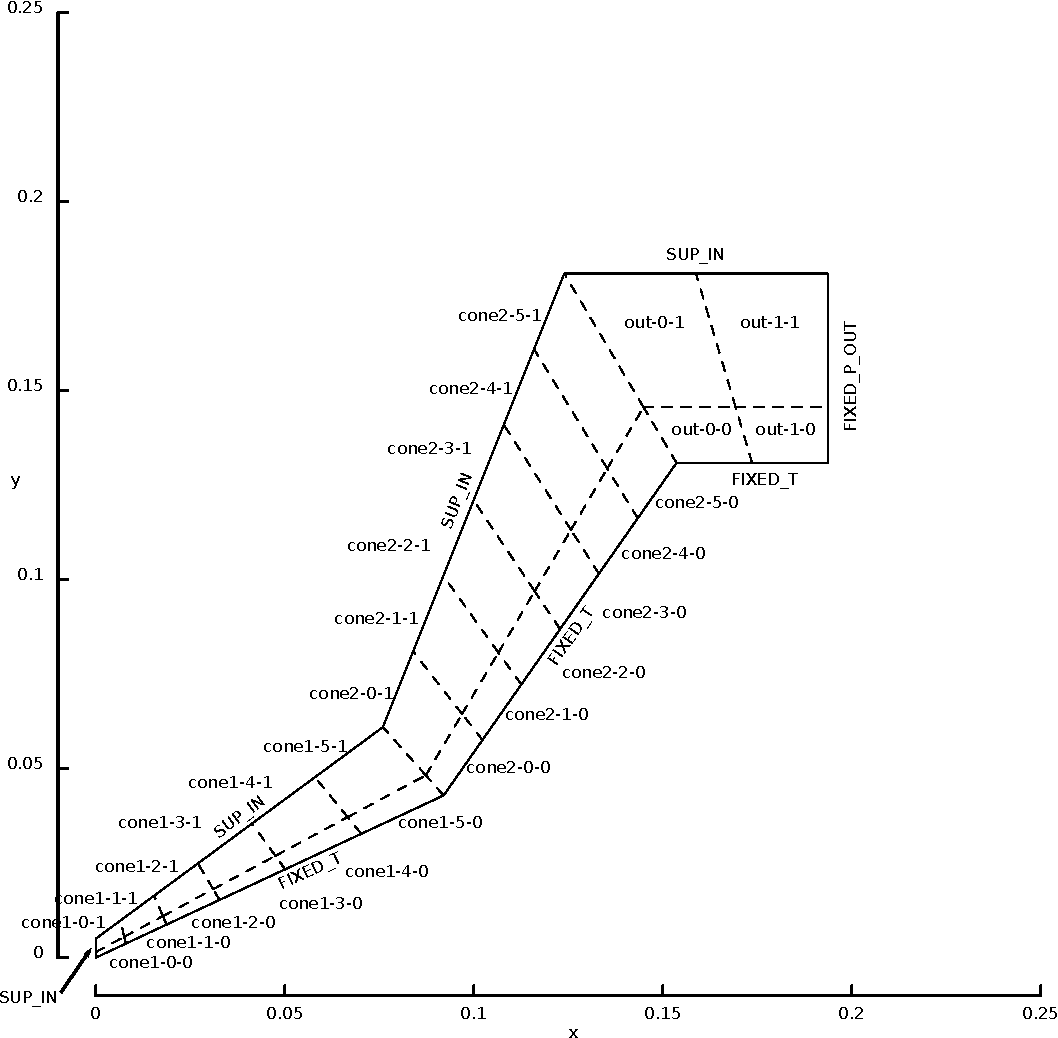
\includegraphics[width=\textwidth,viewport=0 0 430 419,clip=true]{../2D/double-cone-sharp-nose/dbl-cone-edited.pdf}
 \caption{Schematic view of the simulated flow region for the hypersonic flow
          over a double-cone with sharp nose.}
 \label{fig:double-cone-sharp-nose-geometry}
\end{figure}

\medskip
In terms of required computer time, this simulation is more demanding than the cylinder-flare example.
The job scipts submitted to the batch system are shown below.
The preparation of the grids and initial flow-state files was done on a local workstation, 
these files transferred to the cluster computer file system (``arcus'', located at the Oxford e-Research Centre)
and then the simulation was done in two stages, 
0--1.75\,ms and 1.75\,ms--3\,ms.
Note that the 28 blocks have been grouped, via the mpimap file 
(that was generated by the e3loadbalance program), to 14 MPI tasks.
The first simulation stage required just over two days on 14 cores of the arcus cluster.

\noindent
\topbar
\lstinputlisting[language={}]{../2D/double-cone-sharp-nose/prep.sh}\index{mpimap!example of use}
\bottombar\\
\topbar
\lstinputlisting[language={}]{../2D/double-cone-sharp-nose/run-arcus.sh}\index{PBS batch system!example of use}
\bottombar\\
\topbar
\lstinputlisting[language={}]{../2D/double-cone-sharp-nose/run-arcus-2.sh}
\bottombar\\

\clearpage
\subsection{Results}
%
Figure\,\ref{fig:double-cone-sharp-nose-field-data} shows some of the flow field data at $t$=3\,ms after flow start.
The leading shock from the sharp tip of the cone and the shock caused by the boundary-layer separation 
are both clearly defined and can be seen to merge in the pressure field.
This combined shock interacts strongly with the flow up the second cone surface and a Mach stem is formed 
on top af a supersonic jet running up along the cone surface.
The Mach number field, rescaled to highlight the subsonic regions, shows clearly the separation region in the
junction between the conical surfaces, the large subsonic region behind the curved shock over the second cone, 
and the supersonic jet up the surface of that cone.

\begin{figure}[htb]
 \centering
 \subfloat[Pressure field.]{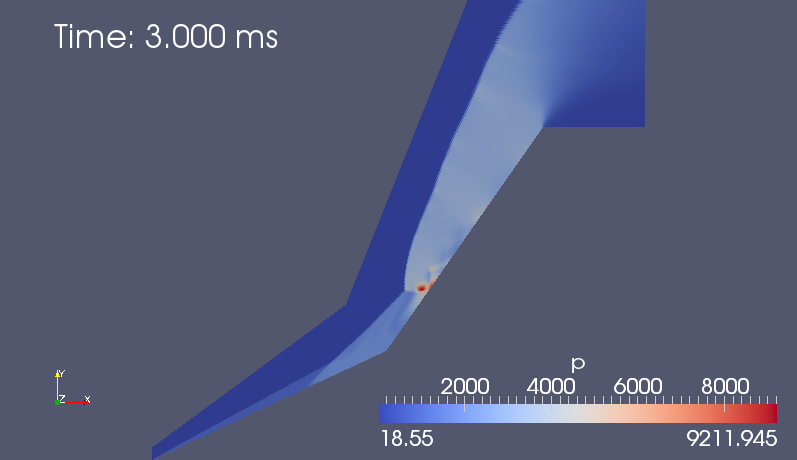
\includegraphics[width=0.5\textwidth]
    {../2D/double-cone-sharp-nose/p-field-3p000ms-factor-2.png}\label{fig:double-cone-sharp-nose-pressure}}
 \subfloat[Mach number.]{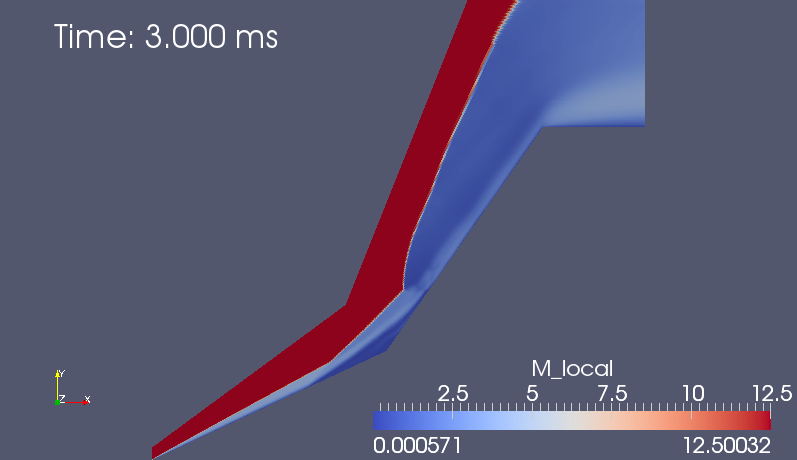
\includegraphics[width=0.5\textwidth]
    {../2D/double-cone-sharp-nose/mach-field-3p000ms-factor-2.png}\label{fig:double-cone-sharp-nose-mach}}\\
 \subfloat[Temperature field.]{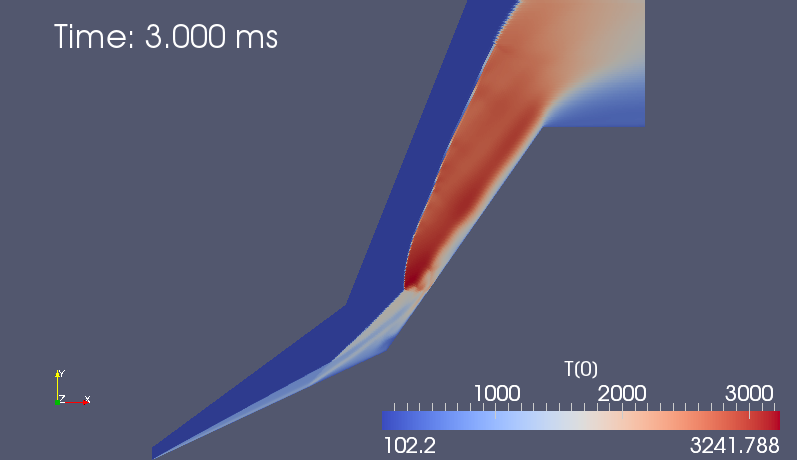
\includegraphics[width=0.5\textwidth]
    {../2D/double-cone-sharp-nose/T-field-3p000ms-factor-2.png}\label{fig:double-cone-sharp-nose-temperature}}
 \subfloat[Mach number rescaled.]{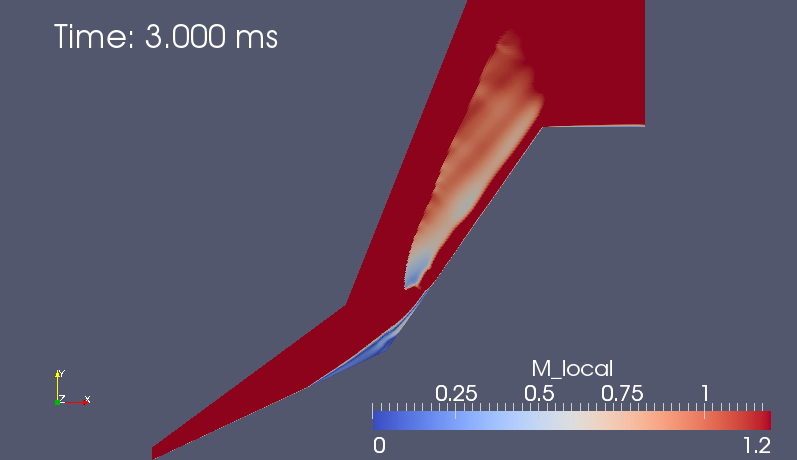
\includegraphics[width=0.5\textwidth]
    {../2D/double-cone-sharp-nose/mach-field-3p000ms-factor-2-subsonic.png}
    \label{fig:double-cone-sharp-nose-mach-subsonic}}
 \caption{Computed flow field at $t$=3\,ms.}
 \label{fig:double-cone-sharp-nose-field-data}
\end{figure}

\medskip
The details of the separation, Mach stem and subsequent jet stream 
are quite complex and some features, such as
shear layers and the shocks within the supersonic jet, are 
more clearly shown by visualizing the gradient of density, as shown in 
Figure\,\ref{fig:double-cone-sharp-nose-grad-density}.
This flow has been more carefully studied in Ref.\cite{nompelis_etal_2003a}.
Here, we are interested only in demonstration how to set up a the simulation
with \texttt{Eilmer} and that the code does indeed produce correct results.

\begin{figure}[htb]
 \centering
 \subfloat[Gradient of density field.]{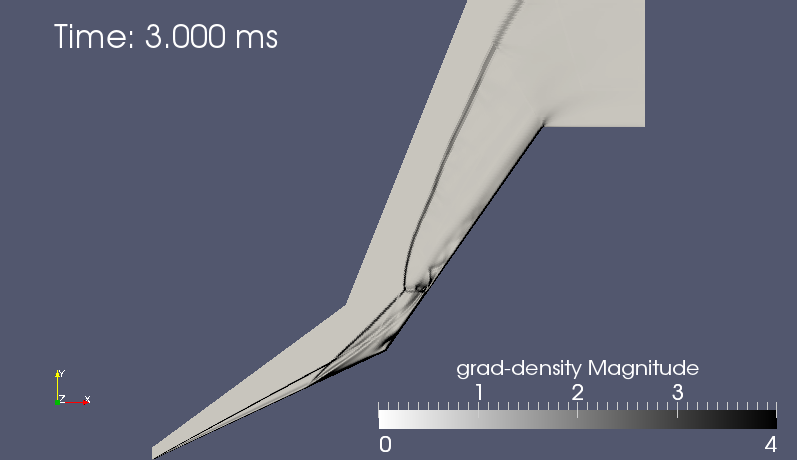
\includegraphics[width=0.7\textwidth]
    {../2D/double-cone-sharp-nose/grad-density-field-3p000ms-factor-2.png}\label{fig:double-cone-sharp-nose-grad-density}}\\
 \caption{Computed flow field at $t$=3\,ms.}
 \label{fig:double-cone-sharp-nose-more-field-data}
\end{figure}


\medskip
By the 3\,ms time shown in Figures\,\ref{fig:double-cone-sharp-nose-field-data} 
and \ref{fig:double-cone-sharp-nose-more-field-data}, 
the flow has settled to a steady-state configuration,
as confirmed by the history of the separation point location on the first conical surface,
plotted in Figure\,\ref{fig:double-cone-sharp-nose-separation-point}.
The data shows a close approach to the asymptotic value of 62.1\,mm by a time of 3\,ms.
The separation point was detected simply as a reversal of the x-velocity, 
as seen in the postprocessing script
in Section\,\ref{double-cone-sharp-nose-post-processing}.

\begin{figure}[htb]
 \centering
 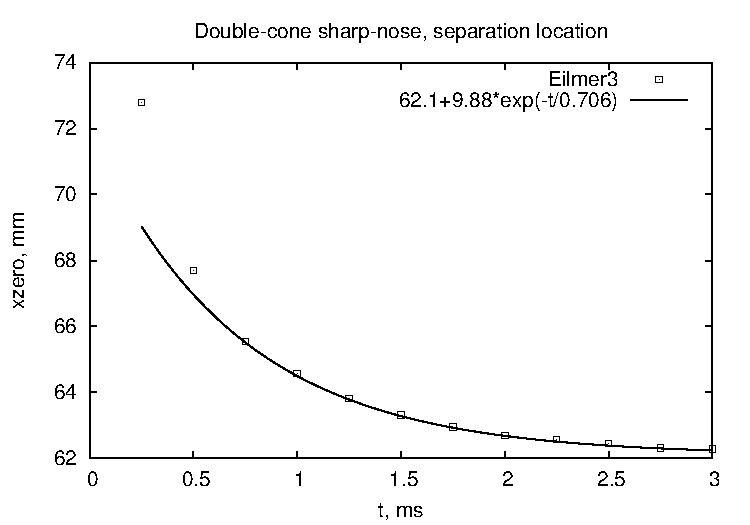
\includegraphics[width=0.7\textwidth]{../2D/double-cone-sharp-nose/separation-location.pdf}
 \caption{History of the separation location along the first conical surface.}
 \label{fig:double-cone-sharp-nose-separation-point}
\end{figure}


\medskip
As another validation case, the real proof of success is in comparison with the experimental data.
Figure\,\ref{fig:double-cone-sharp-nose-plate-data-compare} shows the pressure and heat-transfer
along the surface of both cones.
The plot uses the model axial-coordinate rather than distance along the surface
to match the presentation by MacLean\,\cite{maclean_holden_2004a} and 
the spreadsheet record of data from
the experiments\,\cite{holden_etal_2002a,holden_wadhams_2003a}.
The simulation has done a good job of estimating the pressure distribution right 
through the separation zone and the shock-interaction zone on the second cone's surface.
The separation bubble appears to be well captured in position and extent.

\begin{figure}[htb]
 \centering
 \subfloat[Pressure.]{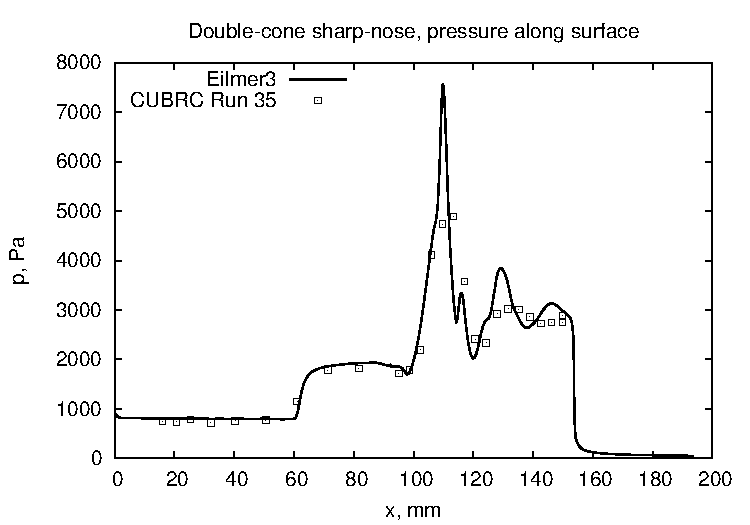
\includegraphics[width=0.5\textwidth]
    {../2D/double-cone-sharp-nose/surface-pressure.pdf}\label{fig:double-cone-sharp-nose-surface-pressure}}
 \subfloat[Heat transfer.]{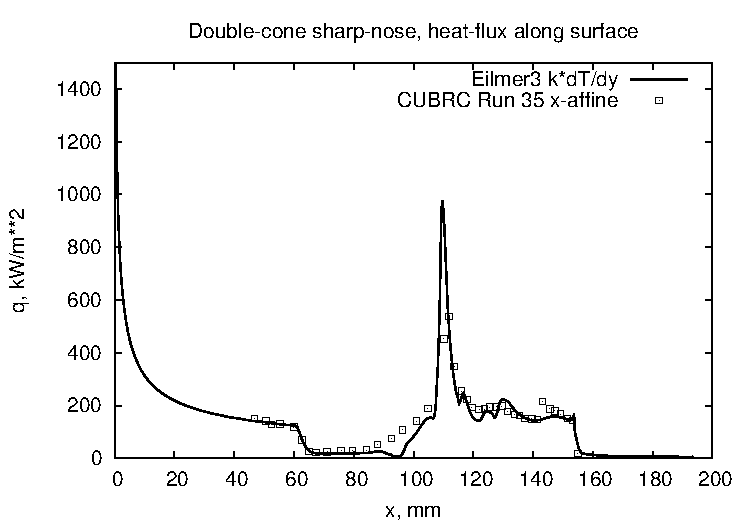
\includegraphics[width=0.5\textwidth]
    {../2D/double-cone-sharp-nose/surface-heat-transfer.pdf}\label{fig:double-cone-sharp-nose-heat-transfer}}
 \caption{Distribution of pressure and heat transfer along the double cone with sharp nose.
   Simulation data is recorded at $t$=3\,ms into the simulation.
   Experimental data is for Run 35 of the CUBRC experiment\,\cite{holden_etal_2002a}.}
 \label{fig:double-cone-sharp-nose-plate-data-compare}
\end{figure}

\medskip
The simulation has also done a good job on the heat transfer estimate,
which has been computed from the field data using the script in Section\,\ref{double-cone-sharp-nose-post-processing}.
It is reassuring that the simulation has accruately captured the heat transfer
in the boundary layer leading into the sepration region,
through the separation, and also after the interaction region on the flare surface.

\clearpage
\subsection{Postprocessing heat transfer and separation-point tracking}
\label{double-cone-sharp-nose-post-processing}
%
The scripts below use the functions imported from \texttt{e3\_flow.py}
at a slightly higher level than in the cone20 example.
The first extracts the data for the cell nearest to the cylinder and flare surface
and uses that data to compute the expected shear stress and heat transfer at the surface.
The second looks at the x-component of the velocity of the first cell above the 
conical surface to identify the location of the start of the separation region
for all frames of the solution.
After writing the location data to a file, it uses the SciPy optimization module 
to fit a simple function to that data, 
in order to estimate the asymptotic position of the separation point for large times.

\noindent
\topbar
\lstinputlisting[language={}]{../2D/double-cone-sharp-nose/dbl_cone_surface_properties.py}
\bottombar

\noindent
\topbar
\lstinputlisting[language={}]{../2D/double-cone-sharp-nose/dbl_cone_separation_point.py}
\bottombar

\subsection{Notes}
\begin{itemize}
 \item The experimental data has come from a spreadsheet, 
 kindly provided by Dr Matthew MacLean of CUBRC.
 Plotting of the pressure was done using dimensional quantities directly with the following GNUPlot script.
 \lstinputlisting[language={}]{../2D/double-cone-sharp-nose/surface-pressure.gnuplot}
 \item The experimental heat transfer data seemed to have incorrect x-positions
 for the transducers.  
 x-position data from the spreadsheet was adjusted to correctly locate the transducer just before
 the separation point and the transducer toward the end of the second-cone surface (as seen in
 the photograph (Figure\,\ref{fig:double-cone-sharp-nose-model}).
 \lstinputlisting[language={}]{../2D/double-cone-sharp-nose/affine.py}
 \item All other heat-transfer transducer locations were then positioned relative to these points.
 \lstinputlisting[language={}]{../2D/double-cone-sharp-nose/surface-heat-transfer.gnuplot}
\end{itemize}
